
\subsection{Background segmentation}


The background segmentation node is based on the backgroundSubtractorMOG2 from OpenCV \cite{BGS} which uses Gaussian mixtures to perform the segmentation. The background segmentation results in a binary image of the foreground. 

\begin{figure}[H]
\begin{center}
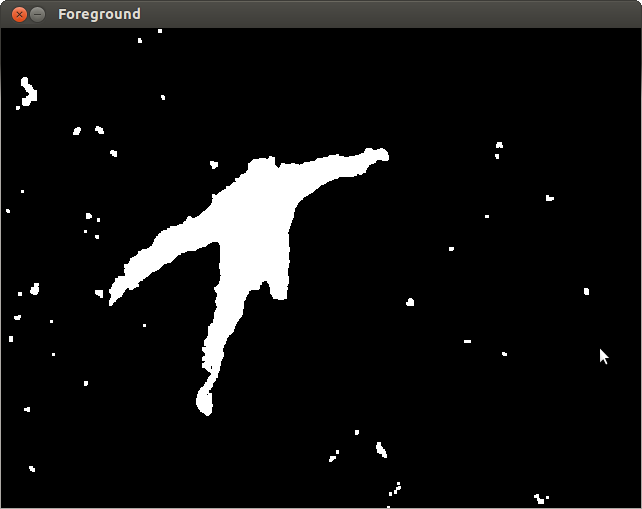
\includegraphics[width=12 cm]{screenshot_foreground_image}
\caption{Foreground from background segmentation}

\end{center}
\end{figure}


The foreground and depth image are used to construct a point cloud. For each foreground pixel the corresponding depth value $P_z$, pixel coordinates $p_x$, $p_y$ and intrinsic parameter can be used to obtain the world coordinates as follows.

\begin{center}
$\displaystyle P_x = (p_x - c_x) \cdot \frac{P_z}{f_x}$\\ \vspace{10 pt}
$\displaystyle P_y = (p_y - c_y) \cdot \frac{P_z}{f_y}$

and the 3D point is ${\bf P} = [P_x, P_y, P_z]^T$
\end{center}


By applying these formulas to all foreground pixels the point cloud is obtained.


